\section{Related work} \label{releatedWork}
This section covers an overview of the material that is the direct foundation for this proposal.

\subsection{Inferred model} \label{inferred-model}
The master thesis by Mulders had two significant outcomes. The first is an inferred model module, and the second is the visualisation of the inferred models. Although the visualisation module becomes required when we want to visualise the result of the change-detection software, it is not necessary to go into depth in this document. This section will discuss what an inferred model is and how they are generated. 

Section \ref{gui-state} the GUI state was discussed. The section ended with the sentence that the universe of states and actions of the SUT's GUI makes up the inferred model. The inferred model is a directed graph showing the GUI-state of the application and its interaction with actions. The vertex of the graph represents the GUI-state. Each vertex has a non-empty set of incoming and outgoing edges, called the actions. 

Figure \ref{fig:state-model} shows the result of the inferred model module.

\bigskip
\begingroup
\captionsetup{type=figure}
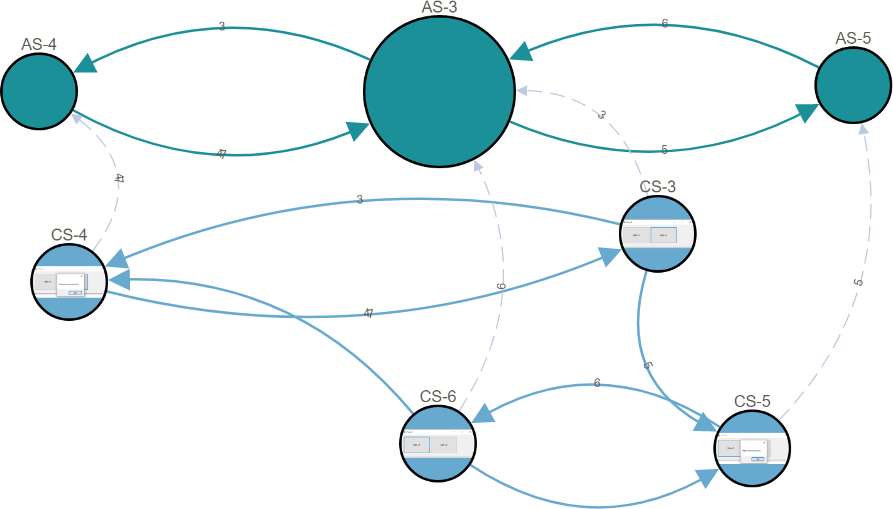
\includegraphics[scale=0.6]{pics/state-model.png}
\captionof{figure}{Inferred model}\label{fig:state-model}
\endgroup

In figure \ref{fig:state-model} two models can be observed. The first model, indicated by the AS text, shows the abstract model. The second, indicated by the CS text, shows the concrete model. 

\subsubsection{Concrete model}
The concrete model contains all the data that could be retrieved from the GUI. The identification key uses a hash calculated over all the properties. Aside from the widget's properties, the concrete models also contain a screenshot of the GUI for each state.

Figure \ref{fig:concrete-node} shows an example of a node in the concrete model. Upon selecting a node, the properties of the node show, including the screenshot taken during the test. The grey dotted line, indicated with the letter 'a', shows the connection with the abstract node, see section \ref{abstract-model} and figure \ref{fig:abstract-node} for more details. The two outcoming edges, indicated with the letter 'b', shows the two actions available in this state. The incoming edge, indicated with the letter 'c', shows how the state was reached. 

\bigskip
\begingroup
\captionsetup{type=figure}
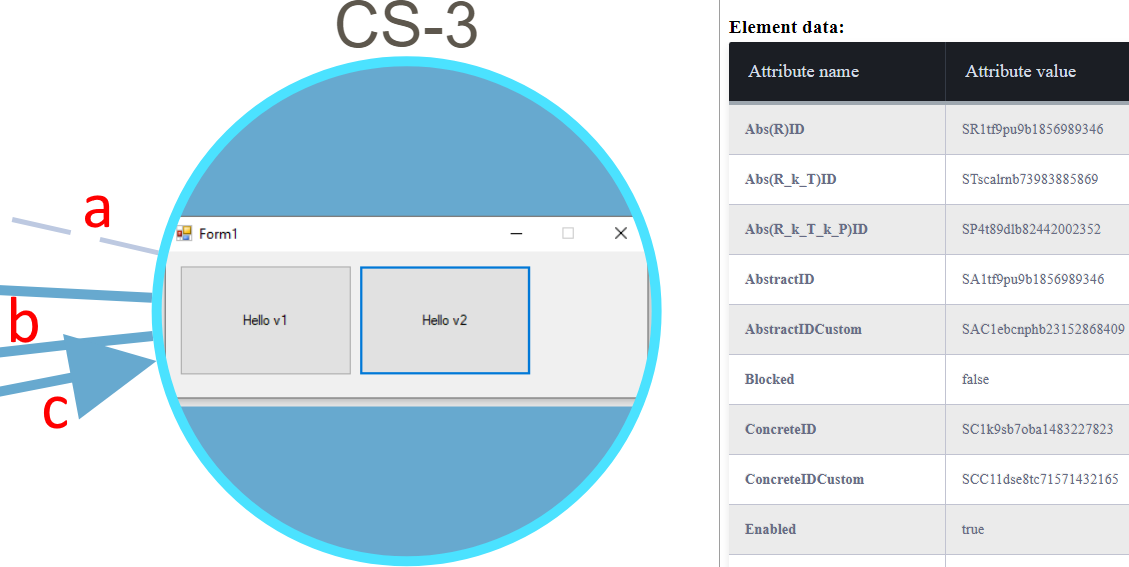
\includegraphics[scale=0.5]{document/pics/concrete-model.png}
\captionof{figure}{A node from the concrete model}\label{fig:concrete-node}
\endgroup

\subsubsection{Abstract model} \label{abstract-model}
Since the concrete models containing all the data from a GUI-state, they can become quite large.  Therefore an abstraction model is made. Figure \ref{fig:abstract-model} shows an example of a node, indicated by 'AS-3'  in the abstract model. The grey lines (from CS-3, CS-6 to AS-3) indicates which concrete state is abstracted. The properties of the abstract node are displayed what the identifier is and which concrete state(s) it represents.

\bigskip
\begingroup
\captionsetup{type=figure}
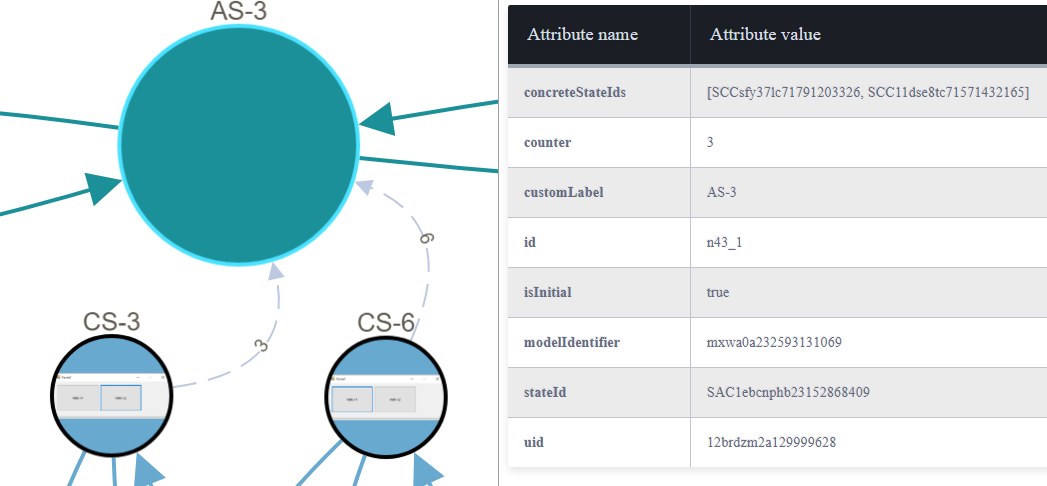
\includegraphics[scale=0.5]{document/pics/abstract-model.png}
\captionof{figure}{A node from the abstract model}\label{fig:abstract-model}
\endgroup

\subsubsection{State identifiers} \label{state-identifiers}
Every state must have a unique id for identification. The identifier is calculated from the information from the widget tree. 

TESTAR uses a hashing algorithm that works as follows: the used properties are concatenated and hashed for each widget. The hashed widget properties are then joined to create a state hash that identifies it. 

To identify the state (and actions), TESTAR calculates two state identifiers; an abstract and concrete state identifier. For the concrete state identifier, all the properties of a widget are used. For the abstract identifier, a subset of the properties is used. It is configurable which properties are used for the abstract identifier. By default the properties \textit{role}, \textit{title}, \textit{position} and \textit{enabled} are used.

When running TESTAR, it is possible to configure which widget properties should be used for the abstract state identifier. Figure \ref{fig:advance} shows the selection dialogue in which the user can select the properties for the abstract id.

\subsubsection{How is an inferred model created?}
This research focuses itself on the outcome of the obtain step as illustrated in figure \ref{fig:obtain-state-graph}, which is the top right part of figure \ref{fig:testart-test-cycle}.

\bigskip
\begingroup
\captionsetup{type=figure}
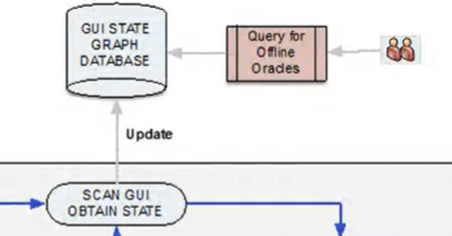
\includegraphics[scale=1]{pics/obtain-state-graph.png}
\captionof{figure}{TESTAR test cycle \cite{VosAho2021}}\label{fig:obtain-state-graph}
\endgroup

Generating the inferred model starts when TESTAR start testing the SUT. After an action has been executed successfully, the state of the GUI is sent to the inferred model module. When the state is sent without an action, it is marked as the initial state. 

The inferred model module generates the abstract and concrete state's and saves those in the model. The model is persisted in the OrientDB database. At last, a model deterministic check is being performed and saved.

\subsection{State model difference}
The \verb|StateModel.Difference| package, added by Pastor Ricós\cite{stateDiff}, offers a proof of concept for calculating differences between the state models. With this proof of concept, the abstract model of two inferred models are compared with each other. For the comparison, the \verb|abstractStateId| is used. 

Pastor Ricós difference algorithm\cite{stateDiff} outputs two classification of changes between two state models: added and removed state. Let $A$ be a set of \verb|abstractStateId|s of version 1 of the SUT, and let $B$ be a set of \verb|abstractStateId|s of version 2 of the SUT. The removed states can be written as
\[A-B = \lbrace x | x \in A \wedge x \notin B \rbrace\]
the states that are added can be written as
\[B-A = \lbrace x | x \in B \wedge x \notin A \rbrace\]

\begingroup
\captionsetup{type=figure}
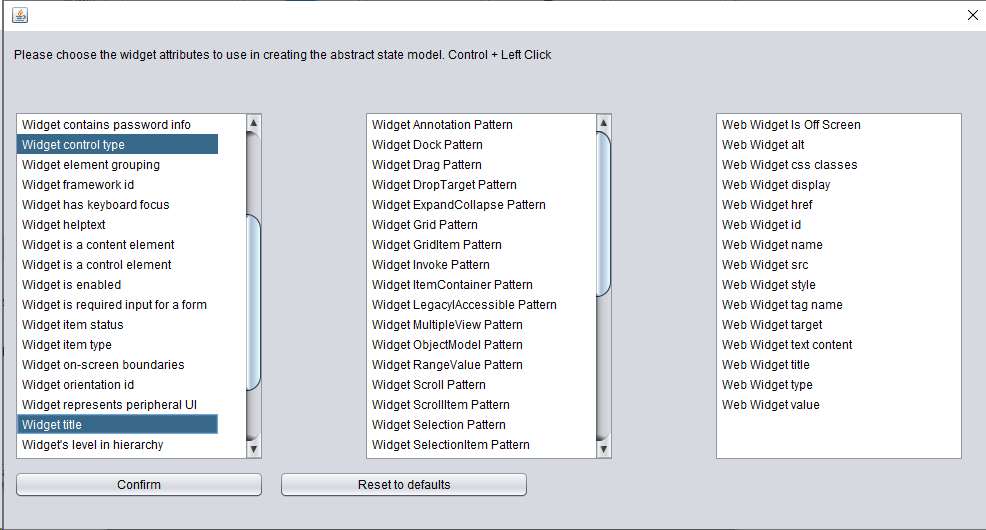
\includegraphics[scale=0.5]{pics/attributes-state-model.png}
\captionof{figure}{Select widgets attributes for the abstractStateId}\label{fig:advance}
\endgroup

Using the \verb|abstractStateId| is excellent for the proof of concept and preliminary change detection, 
However, its boolean nature in which state exists or not can result in many 'false' changes. For example, when a widget is moved, the change detection should result in an altered state, not a removed and added state. 

Section \ref{state-identifiers} discussed how identifiers are generated, since the differences are calculated based on the \verb|abstractStateId| selecting the correct widget attributes is vital. Choosing too few attributes could result in conflicting differences like the same actions are removed and added. Choosing too many attributes could trigger a change in even the tiniest detail, which can be helpful. Choosing the widget attributes can be done with the 'Advance' screen under the State model tab, see Figure \ref{fig:advance}.

For the research proposal, an experiment application is created, the two-buttons app. With the two-buttons app, it was possible to experiment with various TESTAR settings. The application is shown in figures \ref{fig:exp-v1}, \ref{fig:exp-v2} and \ref{fig:exp-v3}. As one can observe, the differences between version 1 and version 2 are the added button with the label 'Hello v2' and between version 2 and 3 the buttons' colour and position. 

\begin{tabularx}{\textwidth}{@{} 
   >{\raggedright\arraybackslash}X
   >{\raggedright\arraybackslash}X  }
    \begingroup
    \captionsetup{type=figure}
    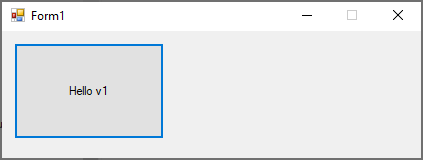
\includegraphics[scale=0.60]{pics/exp-v1.png}
    \captionof{figure}{Version 1 of the experiment application}\label{fig:exp-v1}
    \endgroup
    &
    \begingroup
    \captionsetup{type=figure}
    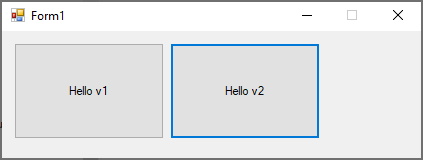
\includegraphics[scale=0.60]{pics/exp-v2.png}
    \captionof{figure}{Version 2 of the experiment application}\label{fig:exp-v2}
    \endgroup
    
    \\
    
    \begingroup
    \captionsetup{type=figure}
    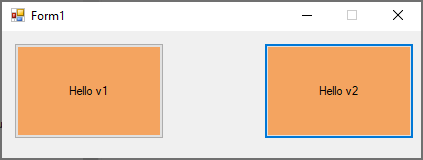
\includegraphics[scale=0.6]{pics/exp-v3.png}
    \captionof{figure}{Version 3 of the experiment application}\label{fig:exp-v3}
    \endgroup
\end{tabularx}

However, a different result is displayed when using 'widget title' and 'widget control type' as widget attributes for the abstract state model. Namely, the button with the label 'Hello v1' is removed between the first two versions, and the buttons labelled 'Hello v1' and 'Hello v2' are added. Between versions 2 and 3, no differences are observed.

Besides change detection on GUI state, the algorithm should also include outgoing actions into consideration. The two-button app experiment shows that selecting different widget properties have an impact on the outcome. However, the algorithm must show that change when an action is removed or leads to another GUI state.   

In the next section (\ref{4.2}), the research questions are discussed. Of course, one of the questions will investigate how the change detection algorithm must be implemented. The findings of the two-button app should be considered, and the experiment should be adapted to contain different changes to test on. 

\subsection{TESTAR in containers}
A recent master thesis by Slomp explains how TESTAR can be integrated into a \acrfull{ci} environment. Slomp introduced TESTAR into the world of Docker and container and integrated TESTAR into an Azure DevOps pipeline. A pipeline is a collection of steps that can automatically build, test and release software. A container bundles all the software, configuration files and libraries together so that an application can run \cite{ms-container}. 

When TESTAR is being run within the Azure DevOps pipeline, the TESTAR GUI is not shown. It is not a problem. However, to analyse the outcome of TESTAR, the users need to install TESTAR and have access to the OrientDB database location. 

By moving the code for change detection and visualisation into a stand-alone web application, the user can analyse the outcome on their browser. Since TESTAR is wrapped into a container, the stand-alone tool will also be wrapped to provide the same infrastructure. Nevertheless, it is up to the IT administrator how they deploy the TESTAR suite. 

Additionally, to the user's benefit, a TESTAR developer can also benefit from the application's separation. Changes to either the separate application or TESTAR can be made without being conflicting with the other. Each tool can focus on one goal, while TESTAR can focus on testing GUI applications. 





Can we leverage image recognition, like with the Murphy tool \cite{murphy-extract-gui}, next to action differences? 

Can it be helpful to make hashes of combined hashes to discover changes or look deeper into underlying hashes, like in a Merkle tree \cite{merkle-tree} structure?